\documentclass[11pt,a4paper,oneside]{report}

\usepackage{graphicx}
\graphicspath{{./images/}}

\usepackage[tmargin=1in,bmargin=1in,lmargin=1.38in,rmargin=0.79in]{geometry}

\usepackage{times}
\usepackage{epsfig}
\usepackage{fancyhdr}
\usepackage{longtable}
\usepackage{subfig}
\usepackage{color}
\usepackage{amsmath}
\usepackage{amssymb}
\usepackage{bm}
\usepackage{tikz}
\usetikzlibrary{arrows.meta,positioning}
\usepackage{psfrag}
\usepackage{url}
\usepackage[linktocpage]{hyperref}

\usepackage[square,numbers]{natbib}

\definecolor{ashgrey}{rgb}{0.7, 0.75, 0.71}

\usepackage{setspace}
\usepackage{multicol}
\usepackage{paralist}
\usepackage{floatrow}

%\setlength{\parindent}{0pt}
\setlength{\parskip}{\baselineskip}
\floatsetup[table]{capposition=top}

\usepackage{titlesec}
\titleformat{\chapter}[block]
{\fontsize{12}{15}\bfseries}
{\thechapter}
{1em}
{\MakeUppercase}
\titlespacing*{\chapter}{0pt}{1pt}{0pt}[0pt]

\titleformat{\section}[block]
{\fontsize{12}{15}\bfseries}
{\thesection}
{1em}
{}
\titlespacing*{\section}{0pt}{0pt}{-12pt}[0pt]

\titleformat{\subsection}[block]
{\fontsize{12}{15}\bfseries}
{\thesubsection}
{1em}
{}
\titlespacing*{\subsection}{0pt}{0pt}{-12pt}[0pt]

\titleformat{\subsubsection}[block]
{\fontsize{12}{15}}
{\thesubsubsection}
{1em}
{}
\titlespacing*{\subsubsection}{0pt}{0pt}{-12pt}[0pt]

\newcommand{\squeezeup}{\vspace{-2.5mm}}
\clubpenalty = 10000
\widowpenalty = 10000

\newcommand{\thesistitle}{Knowledge Distillation with Hierarchical Structural Features for Efficient Object Detection}
\newcommand{\thesisauthor}{Yanshu Zhao}
\newcommand{\thesisprogramme}{Master of Science Dissertation}
\newcommand{\thesisdate}{May 2026}
\newcommand{\thesisyear}{2026}
\newcommand{\thesissupervisor}{Dr. Xiatian Zhu}

\newcommand{\ArchitectureFigure}[2]{
\begin{figure}[t]
\centering
\resizebox{\textwidth}{!}{%
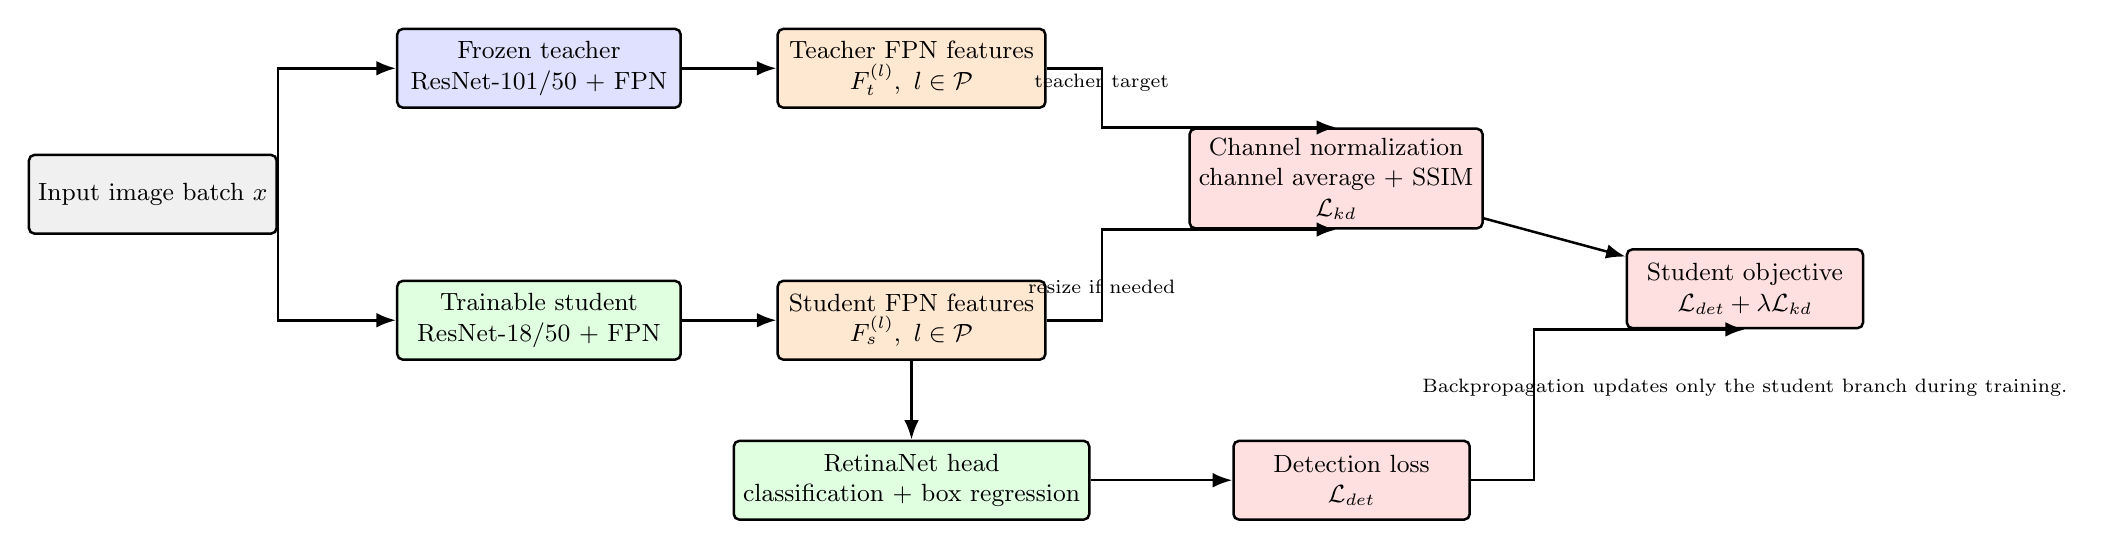
\begin{tikzpicture}[
    font=\small,
    >=Latex,
    line width=0.9pt,
    node distance=8mm and 10mm,
    input/.style={draw, rounded corners=2pt, fill=gray!12, minimum width=28mm, minimum height=10mm, align=center},
    teacher/.style={draw, rounded corners=2pt, fill=blue!12, minimum width=36mm, minimum height=10mm, align=center},
    student/.style={draw, rounded corners=2pt, fill=green!12, minimum width=36mm, minimum height=10mm, align=center},
    feature/.style={draw, rounded corners=2pt, fill=orange!18, minimum width=34mm, minimum height=10mm, align=center},
    loss/.style={draw, rounded corners=2pt, fill=red!12, minimum width=30mm, minimum height=10mm, align=center},
    note/.style={font=\scriptsize, align=center}
]
\node[input] (image) {Input image batch $x$};

\node[teacher, right=15mm of image, yshift=16mm] (teacherbb) {Frozen teacher\\ResNet-101/50 + FPN};
\node[student, right=15mm of image, yshift=-16mm] (studentbb) {Trainable student\\ResNet-18/50 + FPN};
\draw[->] (image.east) |- (teacherbb.west);
\draw[->] (image.east) |- (studentbb.west);

\node[feature, right=12mm of teacherbb] (tfeat) {Teacher FPN features\\$F_t^{(l)},\ l \in \mathcal{P}$};
\node[feature, right=12mm of studentbb] (sfeat) {Student FPN features\\$F_s^{(l)},\ l \in \mathcal{P}$};
\draw[->] (teacherbb) -- (tfeat);
\draw[->] (studentbb) -- (sfeat);

\node[student, below=10mm of sfeat] (head) {RetinaNet head\\classification + box regression};
\draw[->] (sfeat) -- (head);

\node[loss, right=18mm of tfeat, yshift=-14mm] (kd) {Channel normalization\\channel average + SSIM\\$\mathcal{L}_{kd}$};
\draw[->] (tfeat.east) -- ++(7mm,0) |- node[pos=0.28, above, font=\scriptsize] {teacher target} (kd.north);
\draw[->] (sfeat.east) -- ++(7mm,0) |- node[pos=0.28, below, font=\scriptsize] {resize if needed} (kd.south);

\node[loss, right=18mm of head] (det) {Detection loss\\$\mathcal{L}_{det}$};
\draw[->] (head) -- (det);

\node[loss, right=18mm of kd, yshift=-14mm] (total) {Student objective\\$\mathcal{L}_{det} + \lambda \mathcal{L}_{kd}$};
\draw[->] (kd) -- (total);
\draw[->] (det.east) -- ++(8mm,0) |- (total.south);

\node[note, below=5mm of total] {Backpropagation updates only the student branch during training.};
\end{tikzpicture}%
}
\caption{#1}
\label{#2}
\end{figure}
}

\newcommand{\DeepDetectionFigure}{
\begin{figure}[t]
\centering
\resizebox{\textwidth}{!}{%
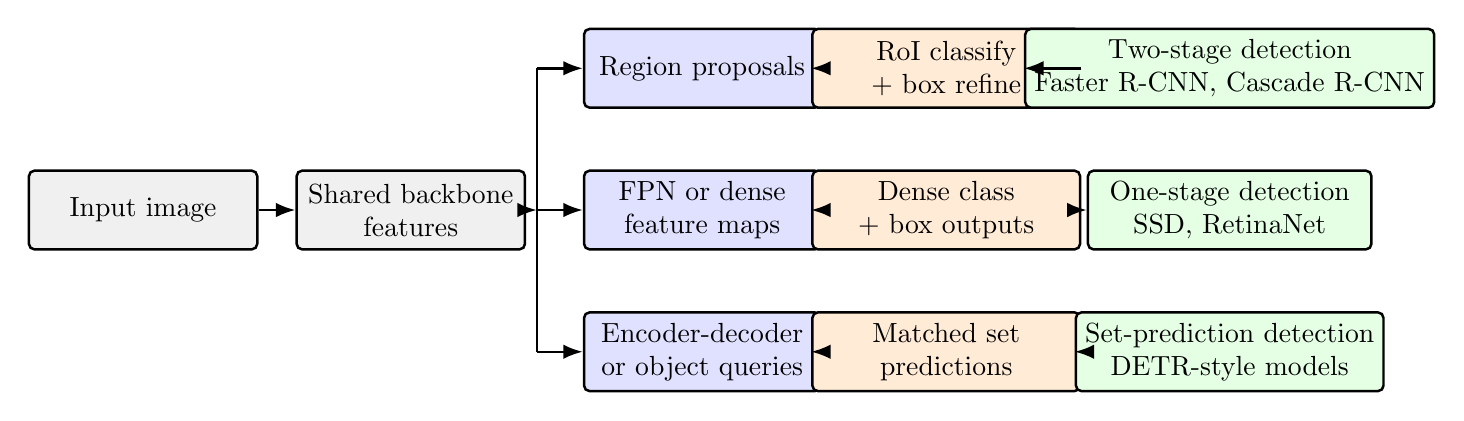
\begin{tikzpicture}[
    font=\normalsize,
    >=Latex,
    line width=0.9pt,
    base/.style={draw, rounded corners=2pt, fill=gray!12, minimum width=29mm, minimum height=10mm, align=center},
    stage/.style={draw, rounded corners=2pt, fill=blue!12, minimum width=30mm, minimum height=10mm, align=center},
    output/.style={draw, rounded corners=2pt, fill=orange!16, minimum width=34mm, minimum height=10mm, align=center},
    family/.style={draw, rounded corners=2pt, fill=green!10, minimum width=36mm, minimum height=10mm, align=center}
]
\node[base] (image) at (0,0) {Input image};
\node[base] (backbone) at (3.4,0) {Shared backbone\\features};
\draw[->] (image) -- (backbone);

\coordinate (split) at (5.0,0);
\draw[->] (backbone.east) -- (split);
\draw (split) -- ++(0,1.8) coordinate (splitTop);
\draw (split) -- ++(0,-1.8) coordinate (splitBot);

\node[stage] (twostagea) at (7.1,1.8) {Region proposals};
\node[output] (twostageb) at (10.2,1.8) {RoI classify\\+ box refine};
\node[family] (twostagenote) at (13.8,1.8) {Two-stage detection\\Faster R-CNN, Cascade R-CNN};
\draw[->] (splitTop) -- (twostagea.west);
\draw[->] (twostagea) -- (twostageb);
\draw[->] (twostageb) -- (twostagenote);

\node[stage] (onestagea) at (7.1,0) {FPN or dense\\feature maps};
\node[output] (onestageb) at (10.2,0) {Dense class\\+ box outputs};
\node[family] (onestagenote) at (13.8,0) {One-stage detection\\SSD, RetinaNet};
\draw[->] (split) -- (onestagea.west);
\draw[->] (onestagea) -- (onestageb);
\draw[->] (onestageb) -- (onestagenote);

\node[stage] (seta) at (7.1,-1.8) {Encoder-decoder\\or object queries};
\node[output] (setb) at (10.2,-1.8) {Matched set\\predictions};
\node[family] (setnote) at (13.8,-1.8) {Set-prediction detection\\DETR-style models};
\draw[->] (splitBot) -- (seta.west);
\draw[->] (seta) -- (setb);
\draw[->] (setb) -- (setnote);
\end{tikzpicture}%
}
\caption{Author's schematic summary of the main deep detection paradigms reviewed in this chapter, based on proposal-based detectors, dense one-stage detectors, and set-prediction transformers \cite{ren2015faster,cai2021cascade,liu2016ssd,lin2017fpn,lin2017focal,carion2020detr}.}
\label{fig:theory-deep-detection}
\end{figure}
}

\newcommand{\IoUFigure}{
\begin{figure}[t]
\centering
\resizebox{0.96\textwidth}{!}{%
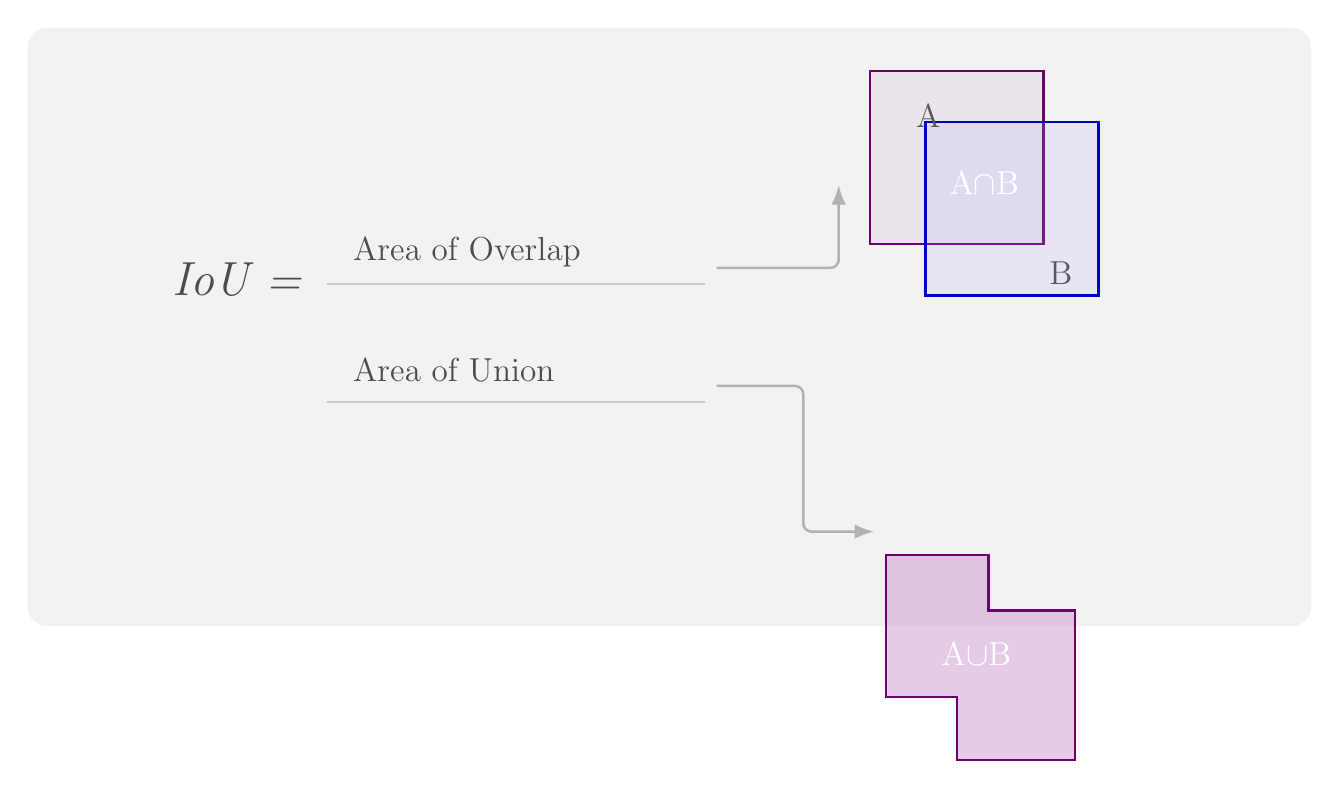
\begin{tikzpicture}[
    font=\normalsize,
    >=Latex,
    line width=0.9pt,
    overlapbox/.style={draw=violet!85!black, fill=violet!35, fill opacity=0.18, text opacity=1, minimum width=22mm, minimum height=22mm, align=center},
    comparebox/.style={draw=blue!80!black, fill=blue!35, fill opacity=0.16, text opacity=1, minimum width=22mm, minimum height=22mm, align=center},
    explabel/.style={font=\large, text=black!70},
    unionfill/.style={fill=violet!45, fill opacity=0.45, draw=violet!85!black}
]
\fill[rounded corners=7pt, gray!10] (-0.6,-3.2) rectangle (15.7,4.4);

\node[anchor=west, text=black!70, font=\fontsize{18}{20}\selectfont\itshape] at (1.1,1.2) {IoU =};
\node[anchor=west, explabel] (overlaptext) at (3.4,1.55) {Area of Overlap};
\draw[black!20, line width=0.7pt] (3.2,1.15) -- (8.0,1.15);
\node[anchor=west, explabel] (uniontext) at (3.4,0.05) {Area of Union};
\draw[black!20, line width=0.7pt] (3.2,-0.35) -- (8.0,-0.35);

\node[overlapbox, anchor=center] (abox) at (11.2,2.75) {};
\node[comparebox, anchor=center] (bbox) at (11.9,2.1) {};
\node[anchor=north west, font=\large, text=black!65] at (10.55,3.55) {A};
\node[anchor=south east, font=\large, text=black!65] at (12.8,1.0) {B};
\node[font=\large, text=white] at (11.55,2.42) {A$\cap$B};

\draw[rounded corners=3pt, black!30, ->] (8.15,1.35) -- (9.7,1.35) -- (9.7,2.4);
\draw[rounded corners=3pt, black!30, ->] (8.15,-0.15) -- (9.25,-0.15) -- (9.25,-2.0) -- (10.15,-2.0);

\begin{scope}[shift={(10.3,-2.3)}]
  \fill[unionfill] (0,0) -- (1.3,0) -- (1.3,-0.7) -- (2.4,-0.7) -- (2.4,-2.6) -- (0.9,-2.6) -- (0.9,-1.8) -- (0,-1.8) -- cycle;
  \draw[violet!85!black] (0,0) -- (1.3,0) -- (1.3,-0.7) -- (2.4,-0.7) -- (2.4,-2.6) -- (0.9,-2.6) -- (0.9,-1.8) -- (0,-1.8) -- cycle;
  \node[font=\large, text=white] at (1.15,-1.25) {A$\cup$B};
\end{scope}
\end{tikzpicture}%
}
\caption{Geometric interpretation of Intersection over Union: the numerator measures the shared overlap between two boxes, while the denominator measures the total union area covered by either box.}
\label{fig:theory-iou}
\end{figure}
}

\newcommand{\KDPrimerFigure}{
\begin{figure}[t]
\centering
\resizebox{\textwidth}{!}{%
\begin{tikzpicture}[
    font=\normalsize,
    >=Latex,
    line width=0.9pt,
    data/.style={draw, rounded corners=2pt, fill=gray!12, minimum width=22mm, minimum height=12mm, align=center},
    teach/.style={draw, rounded corners=2pt, fill=blue!18, minimum width=14mm, minimum height=34mm},
    stud/.style={draw, rounded corners=2pt, fill=blue!22, minimum width=14mm, minimum height=24mm},
    note/.style={draw, rounded corners=2pt, minimum width=29mm, minimum height=9mm, align=center},
    soft/.style={note, fill=orange!18},
    hard/.style={note, fill=green!18},
    loss/.style={draw, rounded corners=2pt, fill=violet!12, minimum width=28mm, minimum height=9mm, align=center}
]
\node[data] (data) at (0,0) {Training data};

\foreach \x/\y in {-0.35/0.18, -0.12/0.06, 0.12/-0.06, 0.35/-0.18} {
  \draw[fill=green!8, draw=black!20] ($(data.west)+(-1.9+\x,0.15+\y)$) rectangle ++(1.2,1.6);
}

\node[anchor=south] at (4.3,2.45) {\textit{Teacher}};
\node[teach] (t1) at (4.1,0.9) {};
\node[teach] (t2) at (4.45,0.9) {};
\node[teach] (t3) at (4.8,0.9) {};
\node[teach] (t4) at (5.15,0.9) {};
\node[teach] (t5) at (5.5,0.9) {};
\node[teach, minimum height=30mm] (t6) at (5.85,0.9) {};
\node[teach, minimum height=26mm] (t7) at (6.2,0.9) {};
\node[teach, minimum height=22mm] (t8) at (6.55,0.9) {};
\node[teach, minimum height=18mm] (t9) at (6.9,0.9) {};
\node at (5.2,0.9) {pre-trained};

\node[anchor=north] at (4.5,-2.35) {\textit{Student}};
\node[stud] (s1) at (4.25,-1.0) {};
\node[stud] (s2) at (4.6,-1.0) {};
\node[stud] (s3) at (4.95,-1.0) {};
\node[stud] (s4) at (5.3,-1.0) {};
\node[stud, minimum height=20mm] (s5) at (5.65,-1.0) {};
\node[stud, minimum height=16mm] (s6) at (6.0,-1.0) {};
\node at (5.15,-1.0) {to be trained};

\draw[->] (data.east) -- ++(1.0,0) |- (t1.west);
\draw[->] (data.east) -- ++(1.0,0) |- (s1.west);

\node[soft] (soft) at (9.0,1.55) {soft labels\\predictions};
\node[hard] (hard) at (9.0,-1.25) {hard labels\\true label};
\node[soft] (pred) at (7.9,-0.35) {predictions};
\node[loss] (distill) at (9.25,0.4) {distilled knowledge};

\draw[->] (t9.east) -- (soft.west);
\draw[->] (s6.east) -- (pred.west);
\draw[->] (soft.south) -- (distill.north);
\draw[->] (distill.west) -- ++(-0.8,0) |- (pred.north);
\draw[->] (hard.west) -- (pred.east);
\end{tikzpicture}%
}
\caption{Author's redrawn teacher-student overview of knowledge distillation, adapted from Varshney's explanatory primer on knowledge distillation in NLP \cite{varshney2021kdprimer}.}
\label{fig:theory-kd-primer}
\end{figure}
}

\newcommand{\KnowledgeDistillationFigure}{
\begin{figure}[t]
\centering
\resizebox{\textwidth}{!}{%
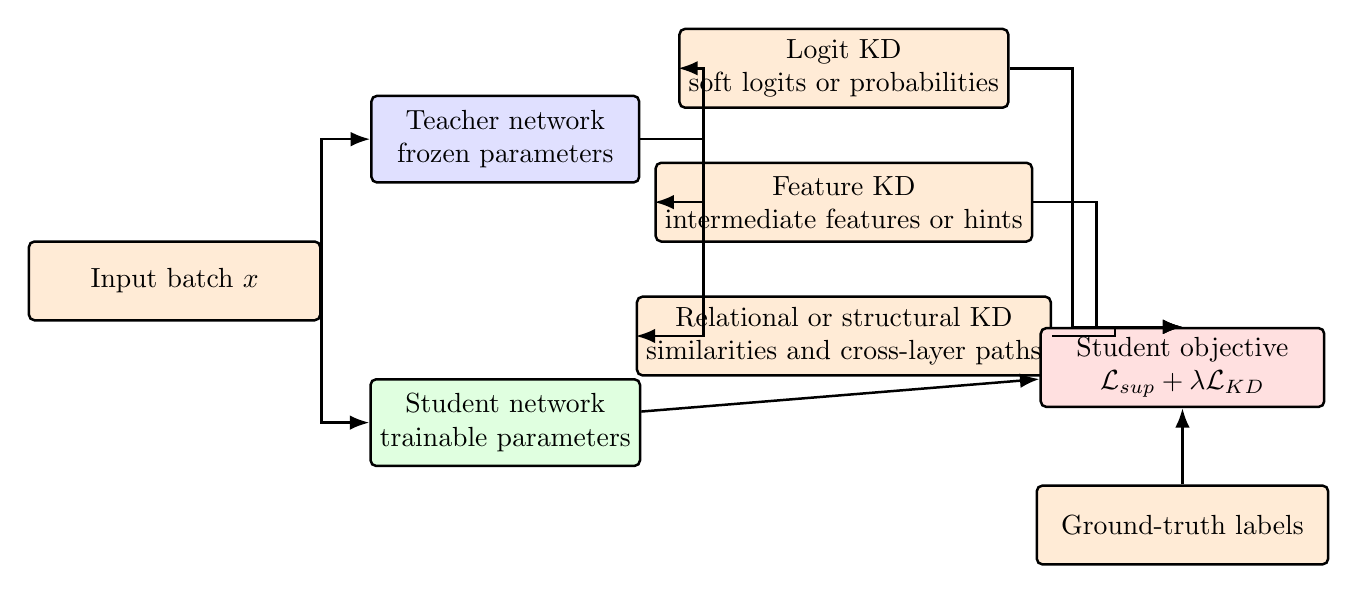
\begin{tikzpicture}[
    font=\normalsize,
    >=Latex,
    line width=0.9pt,
    model/.style={draw, rounded corners=2pt, minimum width=34mm, minimum height=11mm, align=center},
    teacher/.style={model, fill=blue!12},
    student/.style={model, fill=green!12},
    signal/.style={draw, rounded corners=2pt, fill=orange!16, minimum width=37mm, minimum height=10mm, align=center},
    loss/.style={draw, rounded corners=2pt, fill=red!12, minimum width=36mm, minimum height=10mm, align=center}
]
\node[signal] (input) at (0,0) {Input batch $x$};
\node[teacher] (teacher) at (4.2,1.8) {Teacher network\\frozen parameters};
\node[student] (student) at (4.2,-1.8) {Student network\\trainable parameters};
\draw[->] (input.east) |- (teacher.west);
\draw[->] (input.east) |- (student.west);

\node[signal] (logits) at (8.5,2.7) {Logit KD\\soft logits or probabilities};
\node[signal] (features) at (8.5,1.0) {Feature KD\\intermediate features or hints};
\node[signal] (relations) at (8.5,-0.7) {Relational or structural KD\\similarities and cross-layer paths};
\draw[->] (teacher.east) -- ++(0.8,0) |- (logits.west);
\draw[->] (teacher.east) -- ++(0.8,0) |- (features.west);
\draw[->] (teacher.east) -- ++(0.8,0) |- (relations.west);

\node[loss] (objective) at (12.8,-1.1) {Student objective\\$\mathcal{L}_{sup} + \lambda \mathcal{L}_{KD}$};
\draw[->] (student) -- (objective);
\draw[->] (logits.east) -- ++(0.8,0) |- (objective.north);
\draw[->] (features.east) -- ++(0.8,0) |- (objective.north);
\draw[->] (relations.east) -- ++(0.8,0) |- (objective.north);

\node[signal] (labels) at (12.8,-3.1) {Ground-truth labels};
\draw[->] (labels) -- (objective);
\end{tikzpicture}%
}
\caption{Author's schematic view of the common knowledge-distillation pathways discussed in the literature, including logit, feature, cross-layer, and relational transfer \cite{hinton2015distilling,romero2015fitnets,zagoruyko2017paying,yim2017fsp,park2019rkd,chen2021semckd}.}
\label{fig:theory-kd}
\end{figure}
}

\newcommand{\DetectionKDFigure}{
\begin{figure}[t]
\centering
\resizebox{\textwidth}{!}{%
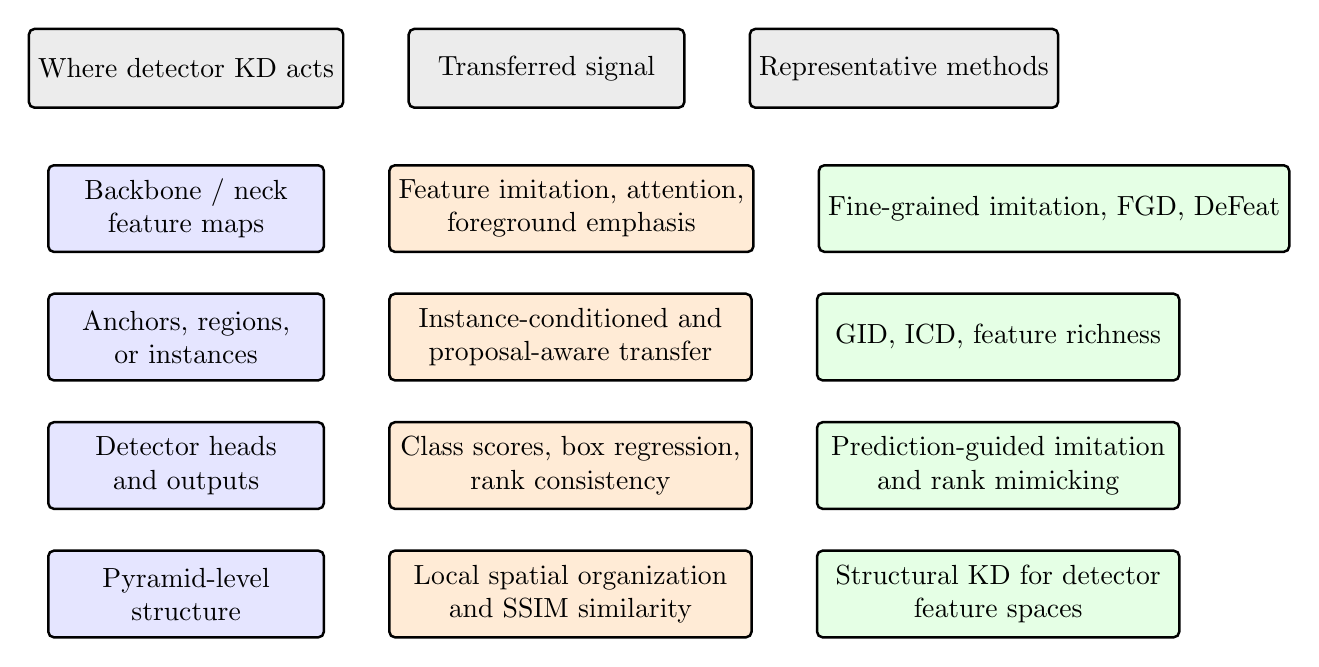
\begin{tikzpicture}[
    font=\normalsize,
    >=Latex,
    line width=0.9pt,
    node distance=9mm and 10mm,
    colhead/.style={draw, rounded corners=2pt, fill=gray!15, minimum width=35mm, minimum height=10mm, align=center},
    leftcell/.style={draw, rounded corners=2pt, fill=blue!10, minimum width=35mm, minimum height=11mm, align=center},
    midcell/.style={draw, rounded corners=2pt, fill=orange!16, minimum width=46mm, minimum height=11mm, align=center},
    rightcell/.style={draw, rounded corners=2pt, fill=green!10, minimum width=46mm, minimum height=11mm, align=center}
]
\node[colhead] (c1) {Where detector KD acts};
\node[colhead, right=8mm of c1] (c2) {Transferred signal};
\node[colhead, right=8mm of c2] (c3) {Representative methods};

\node[leftcell, below=7mm of c1] (r1a) {Backbone / neck\\feature maps};
\node[midcell, right=8mm of r1a] (r1b) {Feature imitation, attention,\\foreground emphasis};
\node[rightcell, right=8mm of r1b] (r1c) {Fine-grained imitation, FGD, DeFeat};

\node[leftcell, below=5mm of r1a] (r2a) {Anchors, regions,\\or instances};
\node[midcell, right=8mm of r2a] (r2b) {Instance-conditioned and\\proposal-aware transfer};
\node[rightcell, right=8mm of r2b] (r2c) {GID, ICD, feature richness};

\node[leftcell, below=5mm of r2a] (r3a) {Detector heads\\and outputs};
\node[midcell, right=8mm of r3a] (r3b) {Class scores, box regression,\\rank consistency};
\node[rightcell, right=8mm of r3b] (r3c) {Prediction-guided imitation\\and rank mimicking};

\node[leftcell, below=5mm of r3a] (r4a) {Pyramid-level\\structure};
\node[midcell, right=8mm of r4a] (r4b) {Local spatial organization\\and SSIM similarity};
\node[rightcell, right=8mm of r4b] (r4c) {Structural KD for detector\\feature spaces};
\end{tikzpicture}%
}
\caption{Author's schematic taxonomy of detector-specific distillation signals, summarizing the main routes emphasized by the object-detection KD literature \cite{wang2019distilling,dai2021gid,guo2021defeat,kang2021icd,du2021frs,li2022rank,yang2022focal,derijk2022structural}.}
\label{fig:theory-detection-kd}
\end{figure}
}

\newcommand{\SSIMDistillationFigure}{
\begin{figure}[t]
\centering
\resizebox{\textwidth}{!}{%
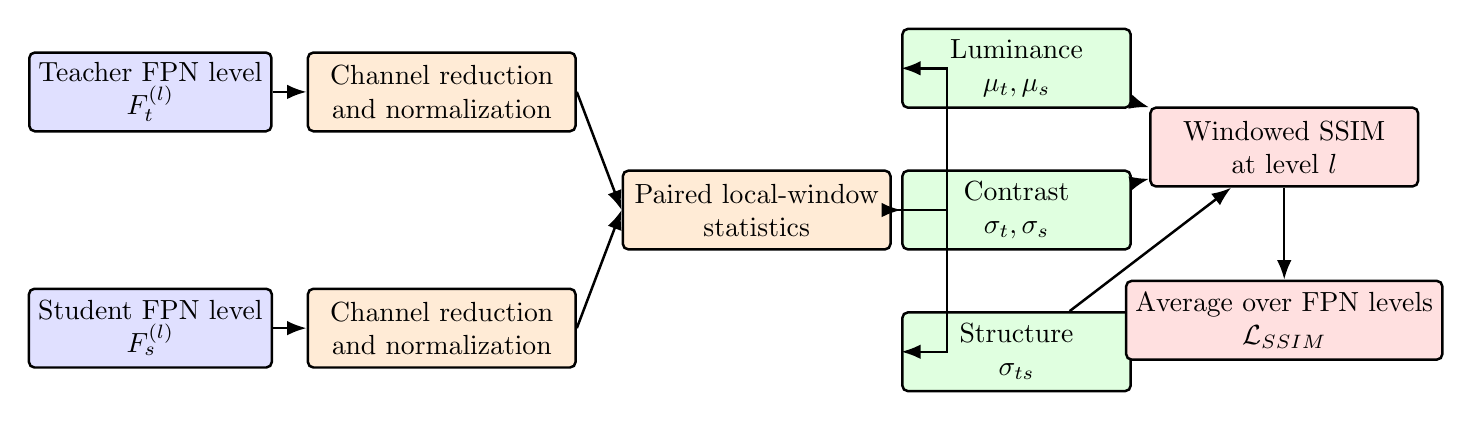
\begin{tikzpicture}[
    font=\normalsize,
    >=Latex,
    line width=0.9pt,
    feat/.style={draw, rounded corners=2pt, fill=blue!12, minimum width=30mm, minimum height=10mm, align=center},
    proc/.style={draw, rounded corners=2pt, fill=orange!16, minimum width=34mm, minimum height=10mm, align=center},
    term/.style={draw, rounded corners=2pt, fill=green!12, minimum width=29mm, minimum height=10mm, align=center},
    loss/.style={draw, rounded corners=2pt, fill=red!12, minimum width=34mm, minimum height=10mm, align=center}
]
\node[feat] (teacher) at (0,1.5) {Teacher FPN level\\$F_t^{(l)}$};
\node[feat] (student) at (0,-1.5) {Student FPN level\\$F_s^{(l)}$};

\node[proc] (tmap) at (3.7,1.5) {Channel reduction\\and normalization};
\node[proc] (smap) at (3.7,-1.5) {Channel reduction\\and normalization};
\draw[->] (teacher) -- (tmap);
\draw[->] (student) -- (smap);

\node[proc] (pair) at (7.7,0) {Paired local-window\\statistics};
\draw[->] (tmap.east) -- (pair.west);
\draw[->] (smap.east) -- (pair.west);

\node[term] (lum) at (11.0,1.8) {Luminance\\$\mu_t,\mu_s$};
\node[term] (con) at (11.0,0) {Contrast\\$\sigma_t,\sigma_s$};
\node[term] (str) at (11.0,-1.8) {Structure\\$\sigma_{ts}$};
\draw[->] (pair.east) -- ++(0.7,0) |- (lum.west);
\draw[->] (pair.east) -- (con.west);
\draw[->] (pair.east) -- ++(0.7,0) |- (str.west);

\node[loss] (ssim) at (14.4,0.8) {Windowed SSIM\\at level $l$};
\node[loss] (total) at (14.4,-1.4) {Average over FPN levels\\$\mathcal{L}_{SSIM}$};
\draw[->] (lum) -- (ssim);
\draw[->] (con) -- (ssim);
\draw[->] (str) -- (ssim);
\draw[->] (ssim) -- (total);
\end{tikzpicture}%
}
\caption{Author's schematic of SSIM-based distillation over aligned FPN features, following the structural-similarity decomposition of luminance, contrast, and structure and its adaptation to detector feature matching \cite{wang2004ssim,wang2003msssim,derijk2022structural}.}
\label{fig:theory-ssim}
\end{figure}
}

\usepackage{style/myfootnote}
\makesavenoteenv{longtable}
\usepackage{vmargin}
\input{./style/epsf.sty}
%%%%%%%%%%%%%%%%%%%%%%%%%%%%%%%%%%%%%%%%%%%%%%%%%%%%%%%%%%%%%%%%%%%%
%%%%%%%%%%%%%%%%%%%%%%%%%%%%%%%%%%%%%%%%%%%%%%%%%%%%%%%%%%%%%%%%%%%%
%        parameters used for page setup and figure placement
%%%%%%%%%%%%%%%%%%%%%%%%%%%%%%%%%%%%%%%%%%%%%%%%%%%%%%%%%%%%%%%%%%%%
%%%%%%%%%%%%%%%%%%%%%%%%%%%%%%%%%%%%%%%%%%%%%%%%%%%%%%%%%%%%%%%%%%%%


%line spacing
\setstretch{1.5}%1.}

%%%%%%%%%%%%%%%%%%%%%%%%%%%%%%%%%%%%%%%%%%%%%%%%%%%%%%%%%%%%%%%%%%%%
% change the allowed picture fractions
%%%%%%%%%%%%%%%%%%%%%%%%%%%%%%%%%%%%%%%%%%%%%%%%%%%%%%%%%%%%%%%%%%%%
\renewcommand{\textfraction}{0.15}
\renewcommand{\topfraction}{0.9}
\renewcommand{\bottomfraction}{0.65}
\renewcommand{\floatpagefraction}{0.6}


%%%%%%%%%%%%%%%%%%%%%%%%%%%%%%%%%%%%%%%%%%%%%%%%%%%%%%%%%%%%%%%%%%%%
% set page dimensions
%%%%%%%%%%%%%%%%%%%%%%%%%%%%%%%%%%%%%%%%%%%%%%%%%%%%%%%%%%%%%%%%%%%%
%put \hoffset = -1in then \oddsidemargin = left margin
%put \voffset = -1in then \topmargin = top margin


%\setmargins{leftmargin}{topmargin}{textwidth}{textheight}{headheight}...
%       {headsep}{footheight}{footskip}
%\setmargins{25mm}{15mm}{160mm}{250mm}{7mm}{7mm}{0pt}{10mm}
\setmargins{40mm}{20mm}{150mm}{235mm}{7mm}{7mm}{0pt}{8mm}
%6.5in15

% DARACH's
%\setlength{\hoffset}{-1.5in}%-1in}
%\setlength{\voffset}{-1.5in}%-1in}
%\setlength{\topmargin}{1.0in}%25in}
%\setlength{\oddsidemargin}{1.5in}
%\setlength{\textwidth}{6.25in}%5.75in}
%\setlength{\textheight}{9.9in}%8.33in}
%\setlength{\headheight}{8pt}%12pt}
%\setlength{\headsep}{20pt}
%\setlength{\footskip}{30pt}%48pt}

%%%%%%%%%%%%%%%%%%%%%%%%%%%%%%%%%%%%%%%%%%%%%%%%%%%%%%%%%%%%%%%%%%%%
%       page header
%%%%%%%%%%%%%%%%%%%%%%%%%%%%%%%%%%%%%%%%%%%%%%%%%%%%%%%%%%%%%%%%%%%%


\pagestyle{fancyplain}
%\renewcommand{\chaptermark}[1]{\markboth{#1}{}}
%\renewcommand{\sectionmark}[1]{\markright{\thesection\ #1}}
\renewcommand{\subsectionmark}[1]{\markright{\thesubsection\ #1}}
\rhead{\fancyplain{}{\bfseries\rightmark}} \lhead{}
    \lhead{}  % TO ADD THE DATE TO THE HEADING, need entry even if empty
    %\lhead{\today}  % TO ADD THE DATE TO THE HEADING, need entry even if empty
\addtocounter{secnumdepth}{1} \addtocounter{tocdepth}{1}


%%%%%%%%%%%%%%%%%%%%%%%%%%%%%%%%%%%%%%%%%%%%%%%%%%%%%%%%%%%%%%%%%%%%

%*********************************
%needed for table and figure captions in minipage
\makeatletter
    \newcommand\figcaption{\def\@captype{figure}\caption}
    \newcommand\tabcaption{\def\@captype{table}\caption}
\makeatother

%%%%%%%%%%%%%%%%%%%%%%%%%%%%%%%%%%%%%%%%%%%%%%%%%%%%%%%%%%%%%%%%%%%%

%                set lengths used in figures

%%%%%%%%%%%%%%%%%%%%%%%%%%%%%%%%%%%%%%%%%%%%%%%%%%%%%%%%%%%%%%%%%%%%

%********************* two image
\newlength{\twoimagevskip}
\setlength{\twoimagevskip}{7pt}

\newlength{\twoimagehskip}
\setlength{\twoimagehskip}{0.03\textwidth} %0.07

\newlength{\twoimagewidth}
\setlength{\twoimagewidth}{0.45\textwidth} %0.4

%********************* three image
\newlength{\threeimagehskip}
\setlength{\threeimagehskip}{8pt}

\newlength{\threeimagevskip}
\setlength{\threeimagevskip}{4pt}

\newlength{\threeimagewidth}
\setlength{\threeimagewidth}{.26\textwidth}


%%%%%%%%%%%%%%%%%%%%%%%%%%%%%%%%%%%%%%%%%%%%%%%%%%%%%%%%%%%%%%%%%%%%

%to raise/lower table values half a box

%%%%%%%%%%%%%%%%%%%%%%%%%%%%%%%%%%%%%%%%%%%%%%%%%%%%%%%%%%%%%%%%%%%%
\newcommand{\up}[1]{\raisebox{1.5ex}[0cm][0cm]{#1}}
\newcommand{\down}[1]{\raisebox{-1.5ex}[0cm][0cm]{#1}}

\newlength{\littlespace}
\setlength{\littlespace}{0.02\textwidth} %0.07

\newlength{\figwidth}
\setlength{\figwidth}{0.6\textwidth} %0.07

\newlength{\figwide}
\setlength{\figwide}{0.8\textwidth} %0.07

\newlength{\twoskip}
\setlength{\twoskip}{0.06\textheight} %0.07

\newcommand{\twodown}[2]{\includegraphics[width=\figwidth]{#1}\vspace{\twoskip}
\includegraphics[width=\figwidth]{#2}\vspace{\twoskip}}

\newlength{\threeskip}
\setlength{\threeskip}{0.03\textheight} %0.07

\newcommand{\onedown}[1]{\includegraphics[width=\figwidth]{#1}\vspace{0.01\textheight}}
\newcommand{\onewide}[1]{\includegraphics[width=\figwide]{#1}\vspace{0.01\textheight}}

\newcommand{\threedown}[3]{\includegraphics[width=\figwidth]{#1}\vspace{\threeskip}
\includegraphics[width=\figwidth]{#2}\vspace{\threeskip}
\includegraphics[width=\figwidth]{#3}\vspace{0.01\textheight}}

\newlength{\fiveskip}
\setlength{\fiveskip}{0.09\textheight} %0.07

\newlength{\fivehoz}
\setlength{\fivehoz}{0.04\textwidth} %0.07

\newlength{\fivewidth}
\setlength{\fivewidth}{0.45\textwidth} %0.07

\newcommand{\fivedown}[5]{\includegraphics[width=\fivewidth]{#1} \hspace{\fivehoz}
\includegraphics[width=\fivewidth]{#2}\vspace{\fiveskip}
\includegraphics[width=\fivewidth]{#3}\hspace{\fivehoz}
\includegraphics[width=\fivewidth]{#4}\vspace{\fiveskip}
\includegraphics[width=\fivewidth]{#5}\vspace{\fiveskip}}


\begin{document}
\normalsize
\rhead{\textcolor{ashgrey}{\thesisauthor, MSc dissertation}}
\renewcommand{\headrulewidth}{0pt}

\begin{center}
{\LARGE {\vspace*{0.5cm}\Huge\bf \thesistitle}}

\vspace{3em}
{\Large \bf \thesisauthor}\\
\vspace{2em}
{\Large\textit{\thesisprogramme}\\
submitted to the\\
University of Surrey\\
\vspace{2em}
\centering
\includegraphics[width=0.6\textwidth]{logo.png}\\
\vspace{2em}
\textit{School of Computer Science and Electrical and Electronic Engineering}\\
Faculty of Engineering and Physical Sciences\\
University of Surrey\\
Guildford, Surrey, GU2 7XH, UK\\
\vspace{2em}
\thesisdate\\
Supervised by: \thesissupervisor\\
\vspace{\stretch{1}}}
\textcopyright \thesisauthor\ \thesisyear
\end{center}
\pagenumbering{roman}

\clearpage
\newpage
\addcontentsline{toc}{chapter}{Declaration of Originality}
\chapter*{Declaration of Originality}
I confirm that the project dissertation I am submitting is entirely my own work and that any material used from other sources has been clearly identified and properly acknowledged and referenced. In submitting this final version of my report to the JISC anti-plagiarism software resource, I confirm that my work does not contravene the university regulations on plagiarism as described in the Student Handbook. In so doing I also acknowledge that I may be held to account for any particular instances of uncited work detected by the JISC anti-plagiarism software, or as may be found by the project examiner or project organiser. I also understand that if an allegation of plagiarism is upheld via an Academic Misconduct Hearing, then I may forfeit any credit for this module or a more severe penalty may be agreed.

\thesistitle

\thesisauthor

Author Signature \hfill Date: \today

\thesissupervisor


\clearpage
\newpage
\addcontentsline{toc}{chapter}{Word Count}
\chapter*{Word Count}

Number of Pages: 61

\noindent Number of Words: Approx.\ 13,500 before final formatting pass


\clearpage
\addcontentsline{toc}{chapter}{Abstract}
\chapter*{Abstract}
This dissertation investigates knowledge distillation for efficient one-stage object detection using RetinaNet. Large detectors with \texttt{ResNet-50} or \texttt{ResNet-101} feature pyramid backbones typically provide stronger representations than lightweight models, but they are substantially more expensive to deploy under practical memory and latency constraints. The central aim of this work is therefore to determine whether a frozen teacher RetinaNet can transfer useful multi-scale structure to a smaller student detector, especially a \texttt{ResNet-18}-based RetinaNet, without increasing inference-time cost.

The proposed method combines the standard RetinaNet detection objective with a feature distillation term applied to aligned FPN representations. Rather than matching raw backbone activations, distillation is performed after the FPN so that teacher and student features already share a common semantic role and a common channel width. This allows the framework to compare selected pyramid levels directly without introducing an additional learned adaptation layer. Structural knowledge transfer is implemented through an SSIM-based loss on normalized, channel-aggregated feature maps, with the goal of preserving local spatial organization that is important for dense object detection.

At the current stage, the dissertation establishes the literature review, architectural design, dimensionality analysis, loss formulation, and COCO-style evaluation protocol needed for the experimental phase. The resulting framework provides a clear basis for comparing student-only RetinaNet training against teacher-guided training and for assessing whether hierarchy-aware structural distillation can improve compact detectors while keeping deployment efficient.


\begin{spacing}{0.1}
\tableofcontents
\end{spacing}

\clearpage
\addcontentsline{toc}{chapter}{List of figures}
\begin{spacing}{1.4}
\listoffigures
\end{spacing}

\newpage
\pagenumbering{arabic}

\pagestyle{fancyplain}
\renewcommand{\headrulewidth}{0pt}
\renewcommand{\footrulewidth}{0pt}

\chapter{Introduction}

Object detection is a core problem in computer vision with applications in autonomous systems, intelligent surveillance, robotics, and medical image analysis. In recent years, deep convolutional detectors have achieved strong accuracy on large-scale benchmarks such as MS COCO, driven by advances in backbone design, multi-scale feature fusion, and improved training objectives \cite{lin2014coco,he2016resnet,lin2017fpn,lin2017focal}. However, the detectors that obtain the highest accuracy often rely on deep backbones and heavy feature extractors, which makes them expensive to deploy in settings with limited memory, latency, or energy budgets. This creates a practical tension: modern detection systems must remain accurate while also becoming efficient enough for real-world inference constraints. More broadly, efficient deployment has also motivated classical model-compression methods such as pruning, quantization, and coding-based compression pipelines \cite{han2015learning,hubara2016quantized,han2016deep}.

One-stage detectors are especially attractive in this context because they offer a clean trade-off between accuracy and speed. RetinaNet is a particularly influential one-stage detector because it combines a Feature Pyramid Network (FPN) with focal loss to address extreme foreground-background imbalance during dense prediction \cite{lin2017fpn,lin2017focal}. Even so, RetinaNet performance depends strongly on the backbone capacity. A detector with a deep \texttt{ResNet-101} feature extractor typically yields better representations than a detector with a lighter \texttt{ResNet-18} backbone, but the latter is preferable when deployment efficiency matters. A natural question is therefore whether the representational strength of a larger RetinaNet can be transferred into a smaller one without reproducing the full computational cost at inference time.

\ArchitectureFigure{Overview of the teacher-student RetinaNet distillation architecture used throughout this dissertation.}{fig:architecture-overview}

\section{Background and Context}

Knowledge distillation offers a principled framework for this goal. In the standard teacher-student setting, a large model is first used as a source of supervision and a smaller student is trained to imitate selected aspects of the teacher while still optimizing the task objective \cite{hinton2015distilling}. Earlier work explored distillation through softened logits, intermediate hints, and attention transfer \cite{romero2015fitnets,zagoruyko2017paying}. In object detection, distillation is more challenging because the model must preserve classification, localization, and multi-scale feature reasoning simultaneously. Recent detection-oriented distillation methods therefore supervise feature maps, spatial relations, and foreground regions rather than relying only on final predictions \cite{wang2019distilling,dai2021gid,guo2021defeat,kang2021icd,du2021frs,li2022rank,yang2022focal}. The continued importance of distillation has even motivated recent work on model provenance, where Shi et al.\ study how to detect whether an open-weights student has been distilled from a teacher under restricted access assumptions \cite{shi2025kddetection}.

This dissertation studies knowledge distillation for efficient one-stage object detection using RetinaNet as the common detection framework. The implemented system uses a frozen teacher detector with a \texttt{ResNet-101} or \texttt{ResNet-50} FPN backbone and trains a smaller student detector, including a \texttt{ResNet-18} configuration, on the same detection task. In addition to the native RetinaNet detection losses, the student is optimized with a feature-based distillation loss applied to FPN representations. Inspired by recent structural knowledge distillation for object detection \cite{derijk2022structural}, the method replaces pointwise feature matching with a structural similarity objective that encourages the student to reproduce the teacher's local spatial organization within the feature pyramid.

The central idea is that feature distillation for detection should preserve not only activation magnitude but also structural relationships that matter for object localization across scales. Structural similarity, originally introduced for image quality assessment, is well suited to this purpose because it compares local statistics such as mean, variance, and correlation rather than treating each activation independently \cite{wang2004ssim}. Building on the SSIM-based distillation perspective of de Rijk et al.\ \cite{derijk2022structural}, this dissertation emphasizes explicit hierarchy-aware supervision over RetinaNet FPN levels so that the student learns teacher structure at multiple resolutions while still being trained end-to-end for dense detection.

\section{Objectives}

The objectives of this dissertation are as follows:

\begin{itemize}
    \item To develop a practical teacher-student distillation framework for RetinaNet with interchangeable ResNet-FPN teacher and student backbones.
    \item To adapt SSIM-based structural distillation to level-aligned FPN features so that multi-scale spatial structure can be transferred directly between detectors.
    \item To analyse the dimensional compatibility of teacher and student features and justify a post-FPN distillation interface that does not require a separate learned adaptation layer.
    \item To implement an evaluation protocol for comparing student-only RetinaNet training with teacher-guided training under COCO-style metrics.
\end{itemize}

\section{Achievements}
% TODO 
The work completed so far has established the main conceptual and technical foundations of the project. A structured review of the literature has been written to position the dissertation within modern detector distillation research. A detailed teacher-student architecture has been formulated for RetinaNet, together with a combined loss that couples standard detection supervision to an SSIM-based feature distillation term. The dissertation also now documents the dimensionality of the teacher and student feature spaces and explains why distillation after the FPN allows direct comparison without an additional adaptation layer. Finally, the training and evaluation protocol has been specified clearly enough to support the next experimental stage of the work.

\section{Practical Considerations and Constraints}

The scope of this dissertation is shaped by a practical but important hardware constraint: experimental training is limited to access to a single rented NVIDIA Tesla V100 GPU with 32 GB of memory, rather than to a dedicated multi-GPU research server \cite{nvidia2017v100}. Although the V100 remains a capable accelerator for deep learning workloads, working within a one-GPU rental budget affects every stage of the study, including feasible image resolution, batch size, training duration, and the number of controlled ablation runs that can be completed within the dissertation timeline. These limits are especially relevant for object detection, where dense prediction, feature pyramids, large backbone activations, and multi-scale supervision collectively create a much heavier memory and compute footprint than standard image classification settings.

Within this context, the choice to study teacher-student distillation with RetinaNet is deliberate rather than merely conservative. RetinaNet provides a strong and well-established one-stage baseline, while its ResNet-FPN design offers a comparatively stable experimental platform for analyzing distillation behaviour \cite{lin2017fpn,lin2017focal}. By keeping the detector family fixed and varying the backbone capacity between teacher and student, the dissertation can focus on the main research question: whether structural feature supervision can transfer useful knowledge from a larger detector to a smaller one under realistic deployment constraints. A more heterogeneous study mixing multiple detector paradigms would make it harder to attribute any observed performance differences specifically to the distillation objective.

This compute budget also limits the ability to explore stronger attention-based detectors in a rigorous way. Transformer-based detection has become an important direction in the literature, with DETR showing that object detection can be formulated through end-to-end set prediction with attention mechanisms \cite{carion2020detr}, and hierarchical transformer backbones such as Swin Transformer becoming competitive general-purpose representations for dense vision tasks \cite{liu2021swin}. These architectures are highly relevant to the broader field, but incorporating them properly would require more than simply swapping one backbone for another. A fair comparison would involve retraining or carefully fine-tuning additional teacher and student configurations, tuning distinct optimization schedules, and repeating the same ablation process across a substantially larger design space. Under a single rented V100, that expansion would consume a large fraction of the available project time and budget before the proposed distillation mechanism itself could be evaluated with sufficient care.

The same constraint applies even more strongly to recent foundation-style detection models. Systems such as GLIP and Grounding DINO combine object detection with language grounding and large-scale multimodal pre-training, thereby moving detection toward open-vocabulary and open-set reasoning \cite{li2022glip,liu2023groundingdino}. GLIP, for example, is pre-trained on 27 million grounding examples, including millions of web-crawled image-text pairs \cite{li2022glip}, while Grounding DINO extends this trend by coupling transformer-based detection with grounded pre-training for arbitrary text-specified categories \cite{liu2023groundingdino}. These models are scientifically important because they greatly broaden what a detector can represent, but reproducing their training pipelines, or even conducting fair fine-tuning studies, would move the dissertation into a very different compute regime. They also introduce extra experimental variables such as language encoders, prompt construction, and pre-training data provenance, which would dilute the present focus on controlled feature distillation for closed-set object detection.

Instead tring to greatly advance SOTA with a more complex architecture, this dissertation focuses on efficiency of smaller detectors through distillation, which is a more tractable and still highly relevant research question under the given constraints. The proposed method can be implemented and evaluated within the available compute budget, while still contributing to the important problem of how to make modern detection systems more efficient for real-world deployment.


% TODO

\section{Overview of Dissertation}

Chapter 2 reviews the background theory and related literature in deep object detection, knowledge distillation, detector-specific distillation, and structural similarity. Chapter 3 presents the proposed methodology, including the problem formulation, the teacher-student architecture, and the dimensional analysis of the feature interface. Chapter 4 details the training objective, FPN feature extraction process, SSIM-based distillation mechanism, and evaluation protocol. Chapter 5 concludes the current draft by evaluating the progress made so far and outlining the most important next steps for the experimental phase.

\chapter{Background Theory and Literature Review}

This chapter reviews the theoretical and research background that motivates the proposed RetinaNet distillation framework. The discussion first considers the evolution of deep object detection, then summarizes the broader knowledge distillation literature, before narrowing to detector-specific distillation methods and the role of structural similarity as a feature-space supervision signal.

\section{Deep Object Detection}

Object detection task is a fundamental problem in computer vision. Modern object detection systems are largely dominated by convolutional and transformer-based deep learning methods, but convolutional detectors remain strong baselines because of their maturity, efficiency, and implementation stability. Two-stage detectors such as Faster R-CNN first generate region proposals and then classify them, while one-stage detectors directly predict dense object hypotheses over feature maps \cite{ren2015faster}. High-quality two-stage localization was later improved further by cascade-style refinement strategies such as Cascade R-CNN, which progressively raises detection quality through multi-stage box refinement at increasing IoU thresholds \cite{cai2021cascade}. One-stage methods historically lagged in accuracy because of severe class imbalance during dense training, but RetinaNet narrowed this gap by introducing focal loss, which down-weights easy negatives and focuses learning on hard examples \cite{lin2017focal}. This made RetinaNet one of the most important foundations for efficient dense detection.

Another key development was the Feature Pyramid Network. FPN constructs semantically strong features at multiple resolutions by combining top-down pathways with lateral connections from the backbone \cite{lin2017fpn}. This design is particularly important in detection because objects vary greatly in scale, and pyramid features allow the detector head to reason across small, medium, and large objects. Since RetinaNet is built on top of FPN features, any distillation strategy for RetinaNet should account for the multi-scale structure of the feature pyramid rather than treating the detector as a single-resolution classifier. Figure~\ref{fig:theory-deep-detection} summarizes the main detector families discussed in this section and highlights where RetinaNet sits within the dense one-stage branch. To make this discussion precise, it is helpful to state the detection task formally.

\begin{figure}[!htp]
  \centering
  \includegraphics[width=0.9\textwidth]{../images/detection.png}
  \caption{Object detection task illustration reproduced from a Wikimedia Commons image by MTheiler (CC BY-SA 4.0) \cite{mtheiler2019yolo}.}
  \label{fig:theory-deep-detection}
\end{figure}

Object detection can be stated as a structured prediction problem over a variable-cardinality set of object instances in an image. Given an input image
\[
  x \in \mathbb{R}^{H \times W \times 3},
\]
the annotation is a set
\[
  y = \{(b_i, c_i)\}_{i=1}^{N},
\]
where $N$ is the number of objects, $b_i = (x_i^{\min}, y_i^{\min}, x_i^{\max}, y_i^{\max})$ denotes an axis-aligned bounding box, and $c_i \in \{1,\dots,C\}$ is the object class label. The learning problem is to estimate parameters $\theta$ of a detector $f_\theta$ such that
\[
  \hat{y} = f_\theta(x) = \{(\hat{b}_j, \hat{s}_j)\}_{j=1}^{M}
\]
approximates the unknown target set well, where $M$ is the number of predicted hypotheses, $\hat{b}_j$ is a predicted box, and $\hat{s}_j \in [0,1]^{C+1}$ is a score vector over $C$ foreground classes plus background. This variable-size prediction view is common across classical region-based detectors, dense one-stage detectors, and newer set-prediction transformers, even though they instantiate candidate generation differently \cite{everingham2010voc,girshick2014rcnn,girshick2015fast,ren2015faster,redmon2016yolo,liu2016ssd,lin2017focal,carion2020detr}.

The main difficulty is that detection must solve localization and recognition jointly. A model must determine whether an object of class $c$ is present, where it is located, and how many instances appear in the image. In practice, modern detectors factor this into a shared feature extractor $\phi_\theta(x)$, often built from deep residual networks \cite{he2016resnet}, followed by detection heads that output class scores and geometric box refinements. For anchor-based detectors, predictions are attached to a dense set of reference boxes or anchors over multiple feature-map locations and aspect ratios, as in SSD and RetinaNet \cite{liu2016ssd,lin2017focal}. For proposal-based detectors, the detector first narrows the search space to a sparse set of candidate regions, then performs per-region classification and regression, as in the progression from R-CNN to Fast R-CNN and Faster R-CNN \cite{girshick2014rcnn,girshick2015fast,ren2015faster}. DETR instead formulates detection as direct set prediction with bipartite matching, reducing reliance on hand-designed anchors and non-maximum suppression heuristics \cite{carion2020detr}. These families differ architecturally, but they all optimize a coupled classification-localization objective over image-conditioned object hypotheses.




For most convolutional detectors, supervision is defined after assigning each candidate prediction to a ground-truth object or to background. This assignment is usually based on Intersection over Union (IoU),
\[
  \operatorname{IoU}(b,\hat{b}) = \frac{|b \cap \hat{b}|}{|b \cup \hat{b}|},
\]
which measures the overlap between two boxes and underlies both training and evaluation \cite{everingham2010voc,lin2014coco,rezatofighi2019giou}. Figure~\ref{fig:theory-iou} gives an intuitive geometric view of this ratio by contrasting the shared intersection region against the full union covered by either box. Let $\mathcal{P}$ denote the set of positive candidates assigned to ground-truth objects and $\mathcal{N}$ the negatives assigned to background. A generic detector loss can then be written as

\IoUFigure

\[
  \mathcal{L}_{\text{det}}
  =
  \frac{1}{|\mathcal{P}|}
  \sum_{k \in \mathcal{P}\cup\mathcal{N}}
  \mathcal{L}_{\text{cls}}(p_k, c_k^\ast)
  \;+\;
  \lambda
  \frac{1}{|\mathcal{P}|}
  \sum_{k \in \mathcal{P}}
  \mathcal{L}_{\text{box}}(t_k, t_k^\ast),
\]
where $p_k$ is the predicted class distribution, $c_k^\ast$ is the assigned class target, $t_k$ is the predicted box parameterization, and $t_k^\ast$ is the regression target. In the R-CNN family, $\mathcal{L}_{\text{box}}$ is commonly instantiated with a Smooth-$L_1$ style regression loss \cite{girshick2015fast,ren2015faster}. In denser one-stage settings, the classification term becomes more delicate because the number of background locations dominates the foreground, which is exactly the imbalance addressed by focal loss in RetinaNet \cite{lin2017focal}. More recent IoU-aware objectives, such as Generalized IoU, further highlight that localization quality should be optimized in a way that is better aligned with the evaluation metric itself \cite{rezatofighi2019giou}.

The need for careful assignment and loss design follows from the fact that detection operates over highly redundant candidate hypotheses. A dense detector may emit thousands of overlapping boxes for a single image, many of which correspond to the same object. Post-processing is therefore typically required to prune duplicates by comparing score-ranked boxes and suppressing those with high mutual overlap. Standard non-maximum suppression has long been part of high-performing pipelines, while Soft-NMS showed that replacing hard removal with continuous score decay can improve recall without changing the detector architecture substantially \cite{girshick2014rcnn,ren2015faster,bodla2017softnms}. Cascade R-CNN can be interpreted as refining this same localization issue during training: rather than using a single IoU threshold, it progressively trains stages at increasing thresholds so that later regressors specialize to higher-quality localization \cite{cai2021cascade}. DETR is an important exception because its one-to-one matching objective aims to avoid duplicate predictions by design \cite{carion2020detr}, but the underlying problem remains the same: the detector must map a large hypothesis space onto a small, correct set of object instances.

A second fundamental challenge is scale variation. Real images may contain large foreground objects, tiny distant objects, heavy clutter, partial occlusion, or extreme aspect ratios. This is one reason deep object detection evolved from early region-based pipelines to multiscale architectures with stronger shared features \cite{girshick2014rcnn,ren2015faster}. FPN addresses this challenge by building semantically meaningful features at multiple resolutions from a common backbone \cite{lin2017fpn}, and this idea strongly influenced both one-stage and two-stage detectors. SSD uses predictions from several feature layers directly \cite{liu2016ssd}, RetinaNet combines dense prediction with FPN and focal loss \cite{lin2017focal}, and modern transformer detectors often still rely on hierarchical or multi-scale representations, whether through pyramidal backbones such as Swin Transformer or through explicit multiscale encoder-decoder designs \cite{liu2021swin,carion2020detr}. In other words, a detector is not simply a classifier applied repeatedly across an image; it is a multiscale structured predictor whose internal representation must preserve semantic discrimination and geometric precision simultaneously.

Evaluation protocols make this formulation concrete. The PASCAL VOC benchmark popularized Average Precision (AP) at a fixed IoU threshold of $0.5$ \cite{everingham2010voc}, whereas MS COCO later adopted the stricter and now standard practice of averaging AP over multiple IoU thresholds from $0.50$ to $0.95$ \cite{lin2014coco}. COCO also reports size-specific metrics for small, medium, and large objects, making clear that localization quality and scale sensitivity are central to detector assessment rather than secondary concerns. These benchmark conventions have shaped model design directly: methods that improve score calibration, box refinement, multiscale features, or suppression behaviour typically translate into better AP because they improve either assignment quality, localization accuracy, or robustness to duplicate predictions \cite{lin2014coco,lin2017fpn,lin2017focal,bodla2017softnms,rezatofighi2019giou}. This benchmark-driven formulation is especially relevant for my project, since RetinaNet itself is trained and evaluated under COCO-style detection metrics.

\section{Knowledge Distillation}

\begin{figure}
  \centering
  \includegraphics[width=0.9\textwidth]{../images/kd.png}
  \caption{Knowledge distillation schematic reproduced from Varshney's primer on knowledge distillation in NLP \cite{varshney2021kdprimer}.}
  \label{fig:theory-kd-primer}
\end{figure}

Knowledge distillation is a general teacher-student learning framework in which a compact model is trained not only against ground-truth labels, but also against supervision derived from a stronger reference model. Earlier model compression work already showed that smaller models can approximate the predictive behaviour of larger ensembles or deeper networks more effectively when they are trained to mimic the teacher function rather than only the hard labels \cite{bucila2006compression,ba2014deep}. The modern formulation was popularized by Hinton et al., who introduced the soft-target objective and the idea of transferring ``dark knowledge'' encoded in the relative probabilities assigned to non-argmax classes \cite{hinton2015distilling}. A standard logit-based distillation objective is
\[
  \mathcal{L}_{\text{KD}}
  =
  T^2\,\mathrm{KL}\!\left(
    \sigma\!\left(\frac{z^t}{T}\right)
    \;\middle\|\;
    \sigma\!\left(\frac{z^s}{T}\right)
  \right),
\]
where $z^t$ and $z^s$ are teacher and student logits, $T$ is the temperature, $\sigma$ is the softmax function, and the $T^2$ term keeps gradients on a comparable scale. In practice this is usually combined with the ordinary supervised loss,
\[
  \mathcal{L}
  =
  (1-\alpha)\,\mathcal{L}_{\text{sup}}
  \;+\;
  \alpha\,\mathcal{L}_{\text{KD}},
\]
so that the student is simultaneously encouraged to fit the data and to approximate the teacher distribution. Survey articles by Gou et al.\ organize this broad literature into output-, feature-, relation-, and response-based categories, which is a useful framing for understanding how the field has evolved beyond vanilla soft labels \cite{gou2021survey}. Figure~\ref{fig:theory-kd} visualizes these common transfer routes in a compact teacher-student schematic.

\KnowledgeDistillationFigure

The most classical and still widely used form is therefore \emph{logit distillation}. Its strength is simplicity: it is architecture-agnostic, easy to add to an existing training loop, and directly exposes inter-class structure that hard labels discard \cite{hinton2015distilling,ba2014deep}. However, later work showed that this approach is not uniformly reliable. In particular, the teacher-student capacity gap matters, and a larger teacher does not automatically imply better transfer \cite{cho2019efficacy}. Mirzadeh et al.\ made this point explicit and proposed \emph{teacher assistant} distillation, where an intermediate-capacity model bridges the mismatch between a very large teacher and a very small student \cite{mirzadeh2020ta}. These results are important because they remind us that distillation is not merely a matter of copying predictions: optimization difficulty, representation mismatch, and training dynamics all affect whether the student can actually exploit the teacher signal.

One major response to the limitations of pure logit matching was the development of \emph{feature distillation}. FitNets proposed using intermediate feature ``hints'' so that thinner or deeper students can imitate hidden teacher representations during training \cite{romero2015fitnets}. Subsequent work argued that not every activation should be matched literally. Attention transfer instead aligns spatial attention maps, aiming to preserve what the teacher attends to rather than every channel value \cite{zagoruyko2017paying}. Neuron Selectivity Transfer interprets the problem as matching distributions of activation patterns via maximum mean discrepancy \cite{huang2017nst}, while Overhaul of Feature Distillation revisits the design of projectors, feature positions, and distance functions in order to make feature imitation more robust and effective \cite{heo2019ofd}. These methods collectively support a key intuition: when the teacher's internal representation is richer than the student's, supervision on intermediate features can guide the student much earlier than output-only KD.

The feature-distillation literature also led naturally to \emph{cross-layer} and \emph{structural} forms of transfer. Rather than assuming that one teacher layer should be paired with one student layer at the same depth, these methods try to preserve how information is organized across layers or stages. Yim et al.\ proposed the Flow of Solution Procedure (FSP) matrix, which encodes the interaction between pairs of layers and thereby distills the flow between representations rather than isolated feature tensors \cite{yim2017fsp}. SemCKD extends this idea by learning attention-based associations between student layers and multiple teacher layers, explicitly addressing the semantic mismatch that arises when networks differ in depth or architecture \cite{chen2021semckd}. Knowledge Review further emphasizes cross-stage pathways and shows that reviewing teacher knowledge through structured intermediate connections can outperform simpler same-level transfer rules \cite{chen2021reviewkd}. Related stagewise training strategies progressively distill one part of the network at a time, improving optimization efficiency and reducing the difficulty of transferring all knowledge in one shot \cite{kulkarni2020skd}. This family is especially relevant to dense prediction, where the hierarchical organization of representations is often as important as any single feature map.

Another influential direction is \emph{relational knowledge distillation}. Instead of requiring the student to reproduce the teacher's absolute coordinates in feature space, relational methods preserve geometry among samples. Park et al.\ proposed Relational Knowledge Distillation (RKD), where the student matches pairwise distances and angles between examples under the teacher representation \cite{park2019rkd}. Similarity-Preserving Knowledge Distillation likewise encourages pairs of samples that are close or far in the teacher feature space to remain close or far in the student space, without forcing the spaces to coincide exactly \cite{tung2019spkd}. Correlation Congruence for Knowledge Distillation extends the same principle to higher-order correlations across mini-batches \cite{peng2019cckd}. The attraction of these approaches is that they preserve structure while allowing the student to realize that structure in its own representation basis, which is often more realistic when teacher and student architectures differ substantially.

More recent methods also cast KD in \emph{information-theoretic} or \emph{contrastive} terms. Variational Information Distillation formulates transfer as maximizing mutual information between teacher and student features, thereby replacing handcrafted similarity objectives with an explicit information criterion \cite{ahn2019vid}. Contrastive Representation Distillation uses the teacher representation as a target in a contrastive objective, encouraging the student to align with the correct teacher feature while separating from negatives \cite{tian2020crd}. These methods are part of a broader shift away from viewing KD as simple regression on logits or activations, and toward viewing it as structured representation learning under teacher guidance.

Taken together, the literature shows that knowledge distillation is best understood as a family of transfer mechanisms rather than a single loss. Logit KD captures class-level dark knowledge, feature KD transfers hidden representations, cross-layer and structural KD preserve hierarchy and connectivity, relational KD preserves geometry between examples, and information-theoretic or contrastive KD focuses on mutual dependence in representation space \cite{gou2021survey}. In my project, this taxonomy matters because object detection depends heavily on multiscale internal features and spatial structure. That makes intermediate, structured, and relation-aware forms of transfer especially appealing, and it helps explain why an SSIM-based feature objective over FPN representations is a sensible design choice for RetinaNet distillation.

\section{Knowledge Distillation for Object Detection}

Detection-specific distillation methods extend the teacher-student paradigm to classification and localization jointly. Chen et al.\ proposed distilling rich feature representations for object detectors and argued that intermediate imitation is more informative than only matching final outputs \cite{chen2017learning}. Wang et al.\ introduced fine-grained feature imitation for dense detectors, emphasizing regions that likely contain objects instead of the entire image uniformly \cite{wang2019distilling}. Dai et al.\ proposed General Instance Distillation (GID), which uses discriminative instance selection to combine feature, relation, and response knowledge more generally across detection frameworks \cite{dai2021gid}. Guo et al.\ proposed Distilling Object Detectors via Decoupled Features (DeFeat), showing that both object and non-object regions can carry useful supervisory information and that distillation can benefit from separating neck-level features from head-level proposal information \cite{guo2021defeat}. Kang et al.\ proposed Instance-Conditional Knowledge Distillation (ICD), which retrieves teacher information conditioned on target instances so that the transfer emphasizes knowledge beneficial to both recognition and localization \cite{kang2021icd}. Du et al.\ then argued that feature selection itself matters, proposing a feature-richness criterion to preserve useful context outside bounding boxes while suppressing misleading background responses \cite{du2021frs}. Li et al.\ studied the discrepancy between teacher and student predictions more directly and proposed rank mimicking together with prediction-guided feature imitation for one-stage detector distillation \cite{li2022rank}. Yang et al.\ proposed Focal and Global Distillation (FGD), which combines foreground emphasis with global contextual transfer to improve detector compression \cite{yang2022focal}. De Rijk et al.\ later proposed structural knowledge distillation, replacing conventional pointwise $\ell_p$ feature matching with an SSIM-based objective for detector feature spaces \cite{derijk2022structural}. Together, these works suggest that successful detection distillation should be spatially aware and should privilege informative regions or structures. Figure~\ref{fig:theory-detection-kd} summarizes the main intervention points that recur across this detector-specific literature.

\DetectionKDFigure

My work is most closely related to the structural distillation framework of de Rijk et al.\ \cite{derijk2022structural}. However, my contribution here is not to introduce FPN itself, which is already central to modern detectors, but to specialize SSIM-based structural distillation to RetinaNet by using level-aligned FPN representations as the main transfer interface between teacher and student. This choice is motivated by two observations. First, the pyramid features of RetinaNet are spatial tensors whose local statistics carry meaningful information about object extent and context at multiple resolutions. Second, a structural measure may preserve teacher organization more faithfully than pointwise losses when student and teacher differ substantially in capacity. The method therefore sits at the intersection of RetinaNet-specific distillation, hierarchy-aware FPN supervision, and structure-aware feature matching.

\section{Structural Similarity as a Distillation Signal}

The Structural Similarity Index Measure (SSIM) was introduced as a perceptual metric for image quality assessment by decomposing local agreement into luminance, contrast, and structural components computed from local means, variances, and covariances \cite{wang2004ssim}. This design is important because it shifts the comparison away from pure pointwise error. Instead of asking whether two patches are numerically identical at each pixel, SSIM asks whether they preserve similar local organization. Multi-scale SSIM later extended this perspective by explicitly evaluating structural fidelity across several resolutions, reflecting the fact that perceptual structure is not tied to a single spatial scale \cite{wang2003msssim}. For feature hierarchies such as FPN, this multi-scale intuition is especially relevant: the same image contains semantically meaningful structure at different resolutions, and a useful distillation signal should not privilege only one of them. Figure~\ref{fig:theory-ssim} illustrates how this decomposition translates naturally into level-wise feature distillation.

\SSIMDistillationFigure

Although SSIM originated in image quality assessment rather than teacher-student learning, the underlying principle transfers naturally to convolutional feature maps. Dense detector features are spatial tensors in which local neighborhoods encode object boundaries, foreground-background transitions, context, and coarse geometry. A loss based only on $\ell_1$, $\ell_2$, or channelwise regression may force the student to copy the teacher's exact activation magnitudes even when the more important requirement is preserving local arrangement. This broader motivation is consistent with work in image restoration and image transformation, where perceptually motivated losses were shown to produce results that better preserve meaningful visual structure than naive per-pixel objectives \cite{zhao2015imgloss,johnson2016perceptual}. At the same time, later work on learned perceptual metrics showed that hand-crafted measures such as SSIM are not the only option, and that deep feature-based distances can better match human judgments in some settings \cite{zhang2018lpips}. Relative to such learned perceptual losses, however, SSIM remains attractive because it is simple, inexpensive, differentiable, and directly interpretable.

These advantages should be understood together with SSIM's limitations. Later analyses showed that SSIM is not a universal notion of perceptual similarity and can behave unintuitively depending on implementation details, local window size, signal range, and averaging conventions \cite{nilsson2020understandssim,venkataramanan2021ssimguide}. This caution is useful for distillation: SSIM should not be treated as a complete replacement for task supervision or as a perfect measure of semantic equivalence. Rather, it is better viewed as a structured regularizer that rewards local statistical agreement between teacher and student. In my work, this interpretation is appropriate because the student is not trained from SSIM alone; it is still optimized under the original detection objective, while SSIM acts as an auxiliary constraint on the internal organization of level-aligned feature maps.

From the perspective of the distillation literature, SSIM also belongs to a broader shift from exact activation imitation toward structure-aware transfer. FSP-based transfer represents knowledge through the interaction between layers rather than through isolated activations \cite{yim2017fsp}. Relational and similarity-preserving methods show that preserving pairwise distances, angles, or correlations between examples can be more realistic than forcing the student into the teacher's exact coordinate system \cite{park2019rkd,tung2019spkd,peng2019cckd}. Structural knowledge distillation for object detection extends this logic most directly to detector features by applying SSIM itself as the transfer objective \cite{derijk2022structural}. The method I propose builds on that insight, but specializes it to RetinaNet's FPN interface. Because both teacher and student expose aligned post-FPN representations with shared spatial semantics, SSIM can be used to compare local structure at each pyramid level without requiring a separate proposal pipeline or a heavily engineered adaptation module.

In this sense, SSIM occupies a useful middle ground for the present problem. It is more geometry-aware than plain pointwise regression, less architecture-dependent than learned perceptual losses based on external classifiers, and better matched to dense detector features than output-only KD. This makes it a reasonable signal when the goal is to preserve the teacher's organization of multiscale feature responses rather than merely its final class probabilities. For RetinaNet distillation, the central hypothesis is therefore not that the student should replicate every teacher activation exactly, but that it should preserve the local structural patterns that support robust dense localization across FPN levels.

\section{Summary}

The literature shows that effective detector distillation must preserve more than final predictions alone. Multi-scale feature representations, foreground-aware transfer, and structure-aware objectives all play an important role in making knowledge transfer useful for dense detection. These observations motivate the methodology developed in the next chapter, which adopts RetinaNet as the common detector family, uses the FPN as the transfer interface, and applies SSIM-based structural supervision to aligned pyramid levels.

\chapter{Methodology}

This chapter introduces the proposed RetinaNet knowledge distillation framework. It first formalizes the training objective, then describes the teacher-student architecture, and finally explains the feature dimensionality choices that make direct structural distillation possible without an additional adaptation layer.

\section{Overview of the Distillation Framework}

Let a teacher detector $T$ and a student detector $S$ operate on an input image $x$ with ground-truth annotations $y$. Both models follow the RetinaNet detection framework, but they may use different ResNet backbones. The goal is to train the student so that it maintains the inference efficiency of a compact detector while recovering part of the representational strength of a larger teacher. During training, the teacher is frozen and serves only as a source of supervisory signals. During inference, only the student is used.

The student is trained with two objectives: the native RetinaNet detection loss and a feature distillation loss. Denoting the student detection loss by $\mathcal{L}_{det}$ and the distillation loss by $\mathcal{L}_{kd}$, the total objective is
\begin{equation}
  \mathcal{L} = \mathcal{L}_{det} + \lambda \mathcal{L}_{kd},
  \label{eq:total-loss}
\end{equation}
where $\lambda$ is a scalar hyperparameter controlling the contribution of distillation. In the implementation used in this project, $\lambda=0.5$ by default.

\section{Teacher and Student Architecture}

Both teacher and student are instantiated as RetinaNet detectors implemented with \texttt{torchvision}. The teacher uses a ResNet-FPN backbone constructed through \texttt{resnet\_fpn\_backbone}, while the student uses either the standard \texttt{retinanet\_resnet50\_fpn} shortcut or a custom RetinaNet built from a lighter ResNet-FPN backbone. This design allows controlled experiments in which the detector head and training framework remain fixed while backbone capacity changes.

\ArchitectureFigure{Architecture of the proposed method. The same transformed input is processed by a frozen teacher and a trainable student, while SSIM-based feature distillation complements the standard RetinaNet detection loss.}{fig:architecture-method}

The teacher branch is configured with a stronger backbone such as \texttt{ResNet-101}, and its parameters are frozen throughout training. The student branch is fully trainable and optimized with backpropagation. Since both models expose pyramid features through the FPN backbone, the framework naturally supports feature-level supervision at selected pyramid levels. In the current implementation, pyramid features are extracted after the input images are processed by RetinaNet's internal transform and backbone modules. If the backbone returns an ordered dictionary of feature maps, those maps are used directly as distillation targets. This choice is important because it defines the interface at which teacher and student are compared: the distillation signal is applied to FPN outputs rather than to raw backbone stages or final detection logits.

\section{Dimensionality and Feature Alignment}

Let the transformed and padded image batch entering the detector be denoted by
\begin{equation}
  x' \in \mathbb{R}^{B \times 3 \times H \times W},
\end{equation}
where $B$ is the batch size and $H \times W$ is the spatial size after RetinaNet preprocessing. Before the FPN, the teacher and student backbones need not have matching internal dimensionality. A bottleneck backbone such as \texttt{ResNet-50} or \texttt{ResNet-101} produces deeper late-stage tensors than a basic-block backbone such as \texttt{ResNet-18}. In practical terms, if one considers the common high-level backbone stages $C3$, $C4$, and $C5$, a bottleneck network exposes channel widths of approximately $(512,1024,2048)$, whereas a lighter \texttt{ResNet-18} exposes approximately $(128,256,512)$. For this reason, direct feature matching on raw backbone outputs would generally require an explicit projection layer, typically a learned $1 \times 1$ convolution, to align student and teacher channels before a loss could be computed reliably.

The proposed method avoids this mismatch by distilling after the FPN rather than before it. The FPN already serves as a built-in dimensionality unifier: each selected backbone stage is projected into a common feature width and fused into a pyramid representation with fixed channel dimension. As a result, for every selected pyramid level $l \in \mathcal{P}$,
\begin{equation}
  F_s^{(l)},\; F_t^{(l)} \in \mathbb{R}^{B \times C \times H_l \times W_l},
\end{equation}
with a shared pyramid width $C=256$ in the standard RetinaNet configuration. The spatial dimensions $H_l$ and $W_l$ depend on the pyramid level rather than on the backbone identity. For the usual RetinaNet levels $P3$ through $P7$, the corresponding strides with respect to the transformed input are $8,16,32,64$, and $128$ pixels, so the feature resolutions decrease systematically as depth increases.

This post-FPN alignment is the main reason no additional adaptation layer is needed between student and teacher features in the present design. The teacher and student already expose tensors with the same semantic role and the same channel dimensionality at each aligned pyramid level. Therefore, the distillation loss can compare level-matched features directly. When a small spatial discrepancy remains because of implementation details or image padding, simple bilinear interpolation is sufficient to align $H_l$ and $W_l$ before computing the loss. No learned adapter is required because the mismatch is not one of feature width or representation type, but only of sampling resolution. Avoiding a trainable adaptation layer also keeps the distillation path lightweight, prevents extra parameters from absorbing part of the knowledge transfer, and makes the empirical comparison with student-only training easier to interpret.

\chapter{Training and Evaluation Framework}

This chapter details how the proposed RetinaNet distillation method is optimized in practice. It describes the standard detection objective, the extraction and alignment of FPN features, the SSIM-based structural loss, and the evaluation protocol that will be used for later experiments.

\section{RetinaNet Detection Loss}

RetinaNet combines classification and box regression losses over dense anchors \cite{lin2017focal}. The classification branch uses focal loss to address the extreme imbalance between background and object anchors. The regression branch predicts bounding-box offsets for positive anchors. In the implementation, the student model returns a dictionary of detection losses, and these terms are summed to form
\begin{equation}
\mathcal{L}_{det} = \mathcal{L}_{cls} + \mathcal{L}_{box},
\end{equation}
where $\mathcal{L}_{cls}$ denotes the focal classification loss and $\mathcal{L}_{box}$ denotes the bounding-box regression loss. This detector objective is identical to standard RetinaNet training and ensures that distillation acts as an auxiliary training signal rather than replacing the detection task.

\section{FPN Feature Extraction}

For an image batch, the teacher and student each produce a set of FPN features
\begin{equation}
\{F_s^{(l)}\}_{l \in \mathcal{P}}, \qquad \{F_t^{(l)}\}_{l \in \mathcal{P}},
\end{equation}
where $\mathcal{P}$ indexes the selected pyramid levels and each feature tensor has shape $B \times 256 \times H_l \times W_l$ after FPN projection. The implementation currently allows distillation on a configurable subset of feature keys, with a default choice focusing on one intermediate pyramid level. Because the comparison is performed after the FPN, the channel dimension is already matched across teacher and student; only the spatial dimensions may occasionally need alignment. When teacher and student produce feature maps with different spatial sizes at the selected level, the student feature is resized by bilinear interpolation to match the teacher resolution before computing the distillation loss.

\section{SSIM-Based Feature Distillation}

The key contribution of the method is a multi-scale structural similarity loss applied to FPN feature maps. For each selected pyramid level $l$, the teacher feature $F_t^{(l)}$ and student feature $F_s^{(l)}$ are first normalized channel-wise using their spatial mean and standard deviation:
\begin{equation}
\hat{F}^{(l)} = \frac{F^{(l)} - \mu(F^{(l)})}{\sigma(F^{(l)}) + \epsilon},
\end{equation}
where $\mu(\cdot)$ and $\sigma(\cdot)$ are computed over the spatial dimensions and $\epsilon$ is a small constant for numerical stability.

After normalization, the feature maps are averaged across channels to obtain a single structural response map per pyramid level:
\begin{equation}
A_s^{(l)} = \frac{1}{C}\sum_{c=1}^{C}\hat{F}_{s,c}^{(l)}, \qquad
A_t^{(l)} = \frac{1}{C}\sum_{c=1}^{C}\hat{F}_{t,c}^{(l)}.
\end{equation}
Consequently, the SSIM comparison is applied to response maps in $\mathbb{R}^{B \times 1 \times H_l \times W_l}$ rather than to the full channel stack. This step reduces sensitivity to channel-wise scale variation and focuses the comparison on shared spatial organization.

The distillation term is then defined as a weighted sum of SSIM losses across the selected pyramid levels:
\begin{equation}
\mathcal{L}_{kd} = \sum_{l \in \mathcal{P}} \alpha_l \, \mathcal{L}_{SSIM}\left(A_s^{(l)}, A_t^{(l)}\right),
\end{equation}
where $\alpha_l$ is the user-defined weight for pyramid level $l$. In practice, the implementation uses the SSIM loss provided by Kornia with a configurable window size, set to $7$ by default. The use of SSIM encourages the student to match teacher feature structure in terms of local intensity patterns, contrast relationships, and spatial correlation. This differs from standard $\ell_1$ or $\ell_2$ matching, which penalize activation differences pointwise and may ignore higher-order local organization.

\section{Training Procedure}

Training proceeds as follows. For each minibatch, the student performs a standard forward pass with detection targets to obtain RetinaNet losses. The teacher then processes the same images in evaluation mode without gradient tracking to produce feature targets. Student FPN features are extracted from the same transformed inputs, the SSIM-based distillation loss is computed, and the combined loss in Eq.~(\ref{eq:total-loss}) is backpropagated only through the student. This keeps optimization efficient and ensures that the teacher remains fixed.

The framework supports both distillation training and student-only training through configuration. When knowledge distillation is disabled, the system reduces to ordinary RetinaNet optimization. When distillation is enabled, the optimizer is applied only to the trainable student parameters. The current implementation supports AdamW and SGD, periodic COCO evaluation, TensorBoard logging, and per-epoch subset sampling. Subset sampling is useful for controlled experiments because it reduces computational cost while preserving the same training code path across runs.

\section{Evaluation Protocol}

Evaluation is conducted with COCO-style metrics using \texttt{pycocotools}, including overall bounding-box mean Average Precision (mAP), mAP at IoU thresholds $0.50$ and $0.75$, and scale-specific scores for small, medium, and large objects \cite{lin2014coco}. During evaluation, the framework can report either teacher or student performance, but the primary dissertation setting focuses on the student branch because the teacher is only a training-time aid. Comparisons should therefore be made between a student trained from scratch and the same student trained with teacher-guided feature distillation.

\section{Summary}

Taken together, Chapters 3 and 4 define a complete distillation pipeline for RetinaNet. The method specifies where teacher supervision enters the detector, how features are aligned, how structural similarity is measured, and how the resulting student should later be evaluated under standard object detection metrics.

\chapter{Conclusions}

This dissertation has so far established the conceptual and methodological basis for studying knowledge distillation in efficient RetinaNet object detection. The current draft now contains a structured introduction to the problem, a focused literature review, a complete teacher-student architectural description, and a formally defined structural distillation objective operating on FPN features. In that sense, the dissertation has moved beyond a general project idea and now documents a coherent framework that can support reproducible experimentation.

\section{Evaluation}

Against the stated objectives, the work completed so far has already achieved several important milestones. First, it defines a practical RetinaNet distillation framework with interchangeable teacher and student backbones, which creates a consistent basis for controlled comparison. Second, it adapts SSIM-based structural distillation to level-aligned FPN representations and explains why this interface is better suited to the task than direct raw-backbone matching. Third, it provides a dimensional analysis of the teacher and student feature spaces, showing clearly why no additional learned adaptation layer is required after the FPN. Fourth, it specifies the combined loss, the optimization pipeline, and the COCO-style evaluation criteria that will be used to assess the method empirically.

The main limitation of the current stage is that the dissertation does not yet report a full set of quantitative experimental results. As a consequence, the strongest contribution at present is the design and justification of the framework rather than a completed empirical comparison. Even so, the methodological groundwork is now sufficiently detailed to support that next phase rigorously.

\section{Future Work}

The most immediate next step is to run the planned experiments and compare student-only RetinaNet training with teacher-guided training across different backbone combinations, especially heavier teachers paired with compact students such as \texttt{ResNet-18}. It will also be important to perform ablation studies on the choice of pyramid levels, the distillation weight $\lambda$, and the SSIM window size in order to understand which design decisions contribute most to performance gains. A further extension would be to compare the present SSIM-based transfer mechanism with simpler pointwise feature losses and with other detector distillation strategies inspired by methods such as FGD and DeFeat. Finally, once quantitative results are available, the dissertation should be expanded with a dedicated analysis of detection accuracy, scale-specific behaviour, and the trade-off between model efficiency and distilled performance.


\addcontentsline{toc}{chapter}{Bibliography}
\bibliographystyle{./style/myabbrvnat}
\bibliography{./references/thesisbib}

\clearpage
\addcontentsline{toc}{chapter}{Appendix}
\chapter*{Appendix}
No appendix material has been added to this dissertation draft yet.


\end{document}
